\documentclass[11pt]{article}
\usepackage{amsmath,amssymb}
\usepackage{graphicx}

\begin{document}

\section{Constructing the first two layers on the three examples}

For each example I construct, in order: the variables, their domains and the schedule; layer $0$; layer $1$ step by step; the sheaf $\mathcal{F}$ on the variables; the dynamics $\Phi$ step by step, following the state $s_t$; and finally how the structure evolves through time. Where the construction required a choice that the definition does not fix, the choice is stated in a footnote.

\subsection{A1. Breadth-first search}

\paragraph{The instances.} Two graphs, with start vertex $s=1$ and neighbours visited in increasing order. The $4$-cycle $C_4$ has vertices $1,2,3,4$ and edges $\{1,2\},\{2,3\},\{3,4\},\{4,1\}$. The domino, two squares sharing an edge, has vertices $1,\dots,6$ and edges $\{1,2\},\{2,3\},\{4,5\},\{5,6\},\{1,4\},\{2,5\},\{3,6\}$.

\paragraph{Variables and domains.} The input is a graph, so its nodes are the input variables, and the state each node carries during the run is its distance: $V_{in}=V=\{1,\dots,n\}$, and the value held by $v$ is $d[v]$.\footnote{Modelling choice: the variable $d[v]$ is identified with the node $v$, so that layer $0$ and layer $1$ live on the same vertices. The alternative keeps the nodes and the distances as separate variables.} The domain of every variable is $D_v=\{0,1,\dots,n-1,\infty\}$, with the two operations the algorithm uses on it, the test $=\infty$ and the successor $x\mapsto x+1$. It is not a field. The queue $Q$ and the current vertex $u$ are not variables: they produce the schedule.\footnote{Modelling choice: $Q$ and $u$ are treated as the schedule. Including them as variables would add a vertex $Q$ touched by every step.}

\paragraph{Schedule.} One step per write $d[w]:=d[u]+1$. A test that finds $d[w]\neq\infty$ writes nothing and is not a step.\footnote{Modelling choice: an operation that writes nothing gives no hyperedge.} On $C_4$: $u=1$ writes $d[2]$ then $d[4]$; $u=2$ writes $d[3]$; $u=4$ and $u=3$ write nothing. So $T=3$. On the domino: $u=1$ writes $d[2],d[4]$; $u=2$ writes $d[3],d[5]$; $u=4$ writes nothing; $u=3$ writes $d[6]$; $u=5,6$ write nothing. So $T=5$.

\paragraph{Layer 0.} The input is a relational structure, so $E_0$ is its own relations, unweighted: $H_0=C_4$ in the first instance and $H_0$ the domino in the second. Every relation of the input is present before the algorithm starts, as Figure 1 shows.

\begin{center}
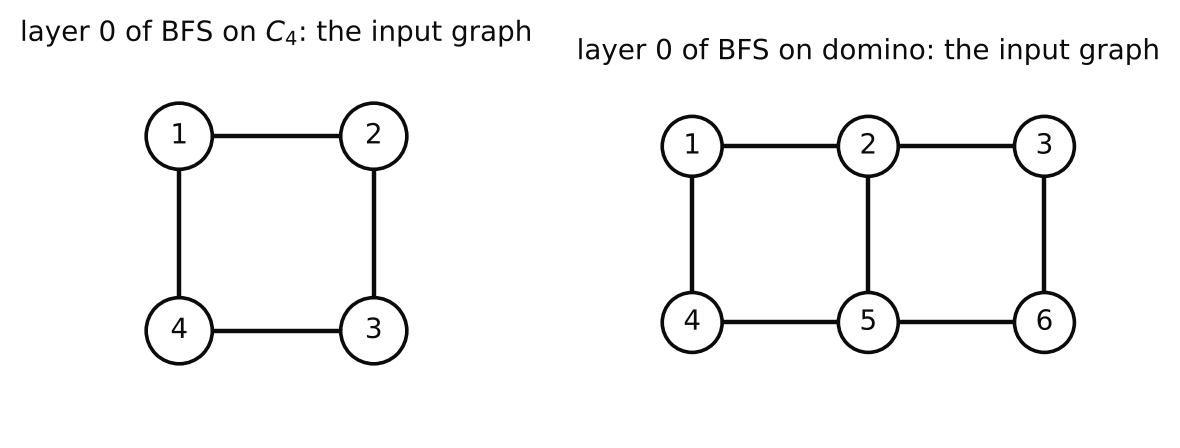
\includegraphics[width=0.75\textwidth]{figs_constructions/bfs_layer0.png}

\textit{Figure 1. Layer 0 of BFS is the input graph itself: its nodes play the role of the inputs and its edges the role of their relations.}
\end{center}

\paragraph{Layer 1.} Each write $d[w]:=d[u]+1$ reads $u$ and $w$ (the test reads $d[w]$, the assignment reads $d[u]$) and writes $w$, so it gives the directed hyperedge $\{u,w\}\to w$ with term \texttt{if d[w]==INF then d[u]+1 else d[w]}. Each snapshot has exactly one hyperedge.

\begin{center}
\begin{tabular}{lll}
\hline
step & $C_4$ & domino\\
\hline
$t=1$ & $\{1,2\}\to2$ & $\{1,2\}\to2$\\
$t=2$ & $\{1,4\}\to4$ & $\{1,4\}\to4$\\
$t=3$ & $\{2,3\}\to3$ & $\{2,3\}\to3$\\
$t=4$ & & $\{2,5\}\to5$\\
$t=5$ & & $\{3,6\}\to6$\\
\hline
\end{tabular}
\end{center}

Figures 2 and 3 draw this table on the graph itself. Each panel is one step $t$: the faint edges are layer $0$, and the orange arrow is the only hyperedge of layer $1$ active at that step, pointing from the vertex read to the vertex written. Reading the panels from left to right is reading layer $1$ along the temporal axis.
\begin{center}
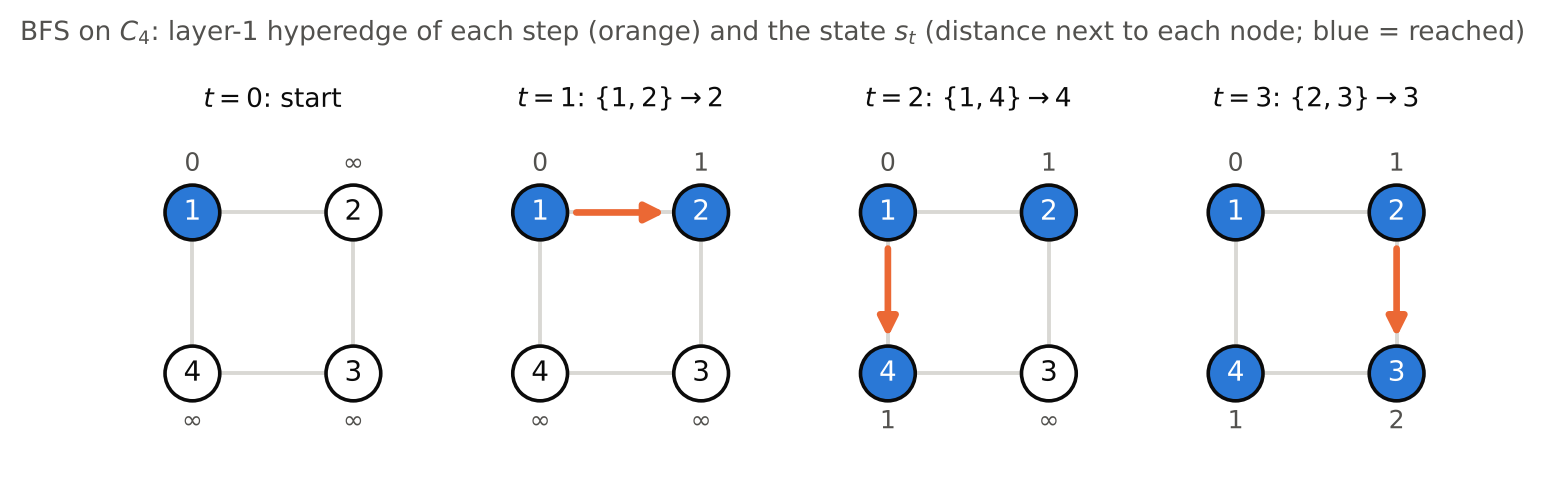
\includegraphics[width=\textwidth]{figs_constructions/bfs_C4_steps.png}

\textit{Figure 2. BFS on $C_4$. Each panel is one time step: the faint graph is layer 0, the orange arrow is the single hyperedge of layer 1 active at that step (from the vertex read to the vertex written), and the number beside each node is its distance in the state $s_t$; blue nodes have been reached.}
\end{center}

\begin{center}
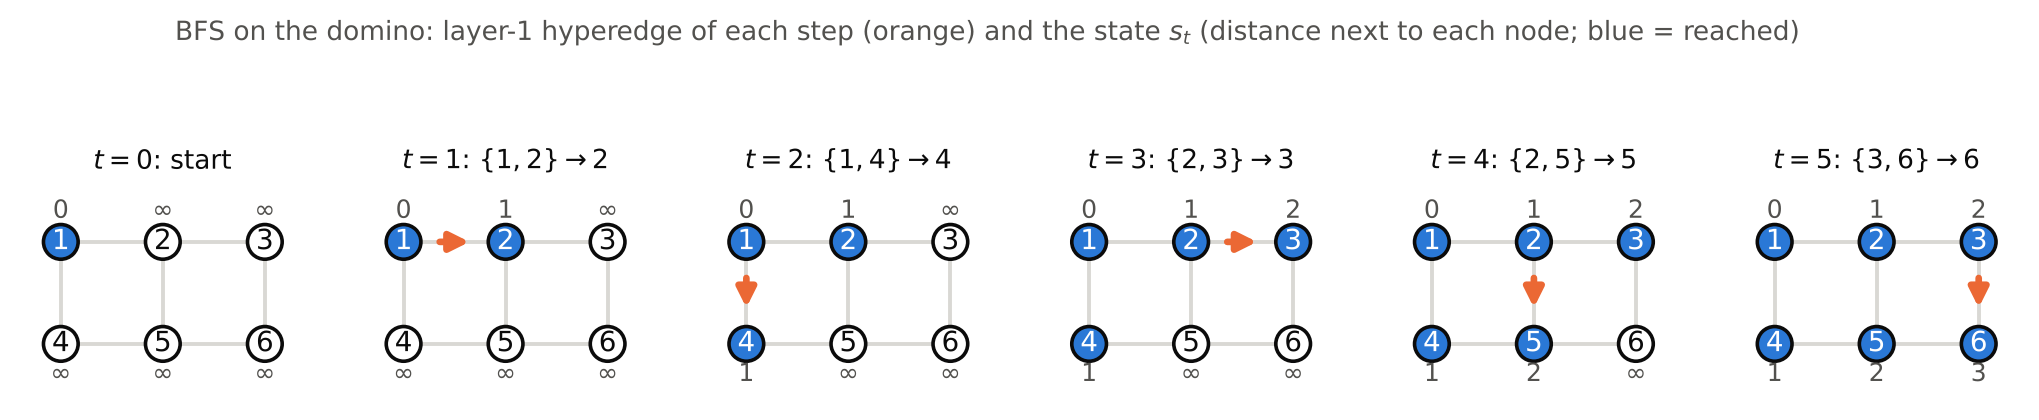
\includegraphics[width=\textwidth]{figs_constructions/bfs_domino_steps.png}

\textit{Figure 3. The same construction on the domino. The edges $\{4,5\}$ and $\{5,6\}$ never carry an orange arrow: both ends were already reached when they were examined.}
\end{center}

\paragraph{The sheaf.} The variables are classical, so $\mathcal{F}(\sigma)$ is the set of probability distributions on $\prod_{v\in\sigma}D_v$, and $\rho_{\sigma\tau}$ is marginalisation. The input is fixed, so every state of the run is a point mass: $s_t=\delta_{d^{(t)}}$, where $d^{(t)}$ is the vector of distances after step $t$, and $s_t|_\sigma=\delta_{d^{(t)}|_\sigma}$. Restricting a point mass just forgets coordinates. In Figures 2 and 3 the state $s_t$ is the column of numbers written beside the nodes, and a node turns blue when its distance leaves $\infty$.

\paragraph{The dynamics.} Each $\Phi_t$ is the single local map $\varphi_o$ that replaces $d[w]$ by $d[u]+1$ and leaves every other coordinate unchanged. On $C_4$:
\[
s_0=\delta_{(0,\infty,\infty,\infty)}\ \xrightarrow{\Phi_1}\ \delta_{(0,1,\infty,\infty)}\ \xrightarrow{\Phi_2}\ \delta_{(0,1,\infty,1)}\ \xrightarrow{\Phi_3}\ \delta_{(0,1,2,1)}.
\]
On the domino:
\[
\delta_{(0,\infty,\infty,\infty,\infty,\infty)}\to\delta_{(0,1,\infty,\infty,\infty,\infty)}\to\delta_{(0,1,\infty,1,\infty,\infty)}\to\delta_{(0,1,2,1,\infty,\infty)}\to\delta_{(0,1,2,1,2,\infty)}\to\delta_{(0,1,2,1,2,3)}.
\]


\paragraph{Evolution through time.} Comparing the first and last panels of Figure 3 summarises the run. Layer $0$ holds every edge of the input from the start. Layer $1$ activates one edge of the input per step, always from a vertex already reached to a vertex not yet reached. The edges activated over the run form the BFS tree: three of the four edges of $C_4$ (not $\{3,4\}$), five of the seven edges of the domino (not $\{4,5\}$ nor $\{5,6\}$). The edges never activated are those whose two ends were both reached before the edge was examined. The sheaf carries no uncertainty at any time.

\subsection{A2. Quantum teleportation}

\paragraph{Variables and domains.} The input variables are the qubits $V_{in}=\{q_0,q_1,q_2\}$, each with domain $\mathbb{C}^2$. The run creates the classical bits $m_1,m_2$ at step $3$ and Bob's copies $m_1',m_2'$ at step $4$, each with domain $\{0,1\}$; they are temporary.\footnote{Following the decision that sending a bit is an operation, Bob's received bits are copies $m_1',m_2'$, distinct from Alice's $m_1,m_2$.} So $V=\{q_0,q_1,q_2,m_1,m_2,m_1',m_2'\}$, $V_0=V_1=V_2=\{q_0,q_1,q_2\}$, $V_3=V_2\cup\{m_1,m_2\}$, and $V_t=V$ for $t\ge4$.

\paragraph{Schedule.} Six steps, the six steps of the protocol: $T=6$.

\paragraph{Layer 0.} The input state is $\rho=|\psi\rangle\langle\psi|\otimes|\beta_{00}\rangle\langle\beta_{00}|$ on $q_0,q_1,q_2$, with $|\beta_{00}\rangle=(|00\rangle+|11\rangle)/\sqrt2$. The candidate hyperedges are the three pairs and the triple.

For the pair $\{q_1,q_2\}$: the reduced state is the pure state $|\beta_{00}\rangle\langle\beta_{00}|$, so $S(\rho_{q_1q_2})=0$, while $\rho_{q_1}=\rho_{q_2}=I/2$ have entropy $1$. Hence $w(\{q_1,q_2\})=1+1-0=2$ bits, the largest value two qubits can share.

For the pairs $\{q_0,q_1\}$ and $\{q_0,q_2\}$: $q_0$ is in the pure state $|\psi\rangle$ and independent of the others, so $\rho_{q_0q_j}=|\psi\rangle\langle\psi|\otimes I/2$ and $w=0+1-1=0$.

For the triple: any state $\sigma$ with the same two-qubit marginals has $\sigma_{q_1q_2}=|\beta_{00}\rangle\langle\beta_{00}|$, a pure state; a state whose marginal on $q_1q_2$ is pure must be a product $\sigma=\sigma_{q_0}\otimes|\beta_{00}\rangle\langle\beta_{00}|$, and $\sigma_{q_0}=|\psi\rangle\langle\psi|$ is forced by the marginal $\sigma_{q_0q_1}$. So $\sigma=\rho$, the maximum-entropy state is $\rho$ itself, and $w(\{q_0,q_1,q_2\})=S(\rho)-S(\rho)=0$.

Layer $0$ is therefore the single edge $\{q_1,q_2\}$ of weight $2$, with $q_0$ isolated, as in the first panel of Figure 5 below. It does not depend on $|\psi\rangle$.

\paragraph{Layer 1.}
\begin{center}
\begin{tabular}{lll}
\hline
step & hyperedges & term\\
\hline
$t=1$ & $\{q_0,q_1\}\to q_1$ & $\mathrm{CNOT}$, control $q_0$, target $q_1$\\
$t=2$ & $\{q_0\}\to q_0$ & $H$\\
$t=3$ & $\{q_0\}\to m_1$,\ \ $\{q_1\}\to m_2$ & measurement in $\{|0\rangle,|1\rangle\}$\\
$t=4$ & $\{m_1\}\to m_1'$,\ \ $\{m_2\}\to m_2'$ & copy over the channel\\
$t=5$ & $\{m_2',q_2\}\to q_2$ & $X^{m_2'}$\\
$t=6$ & $\{m_1',q_2\}\to q_2$ & $Z^{m_1'}$\\
\hline
\end{tabular}
\end{center}
At $t=1$ the CNOT reads both qubits (the new value of the target depends on both) and writes the target, so it is one hyperedge directed from control to target. At $t=3$ the two measurements happen at the same time but are two operations, each reading one qubit, so they are two hyperedges.\footnote{Modelling choice: simultaneous but separate operations give separate hyperedges in the same snapshot.} At $t=5,6$ Bob's corrections read a bit and the qubit and write the qubit. Figure 4 draws the hypergraph $H_1^t$ of each step on the fixed vertex positions of the variables: Alice's qubits and bits on the left, Bob's copies and qubit on the right. A temporary variable appears from the step that creates it. In each panel the shaded region is a hyperedge, the variables it reads are ringed in orange, the variable it writes is filled in orange, and the arrow runs from what is read to what is written; a unary operation such as $H$ is a shaded disc with a loop. The panels $H_1^3$ and $H_1^4$ each contain two hyperedges: the simultaneous but separate operations.

\begin{center}
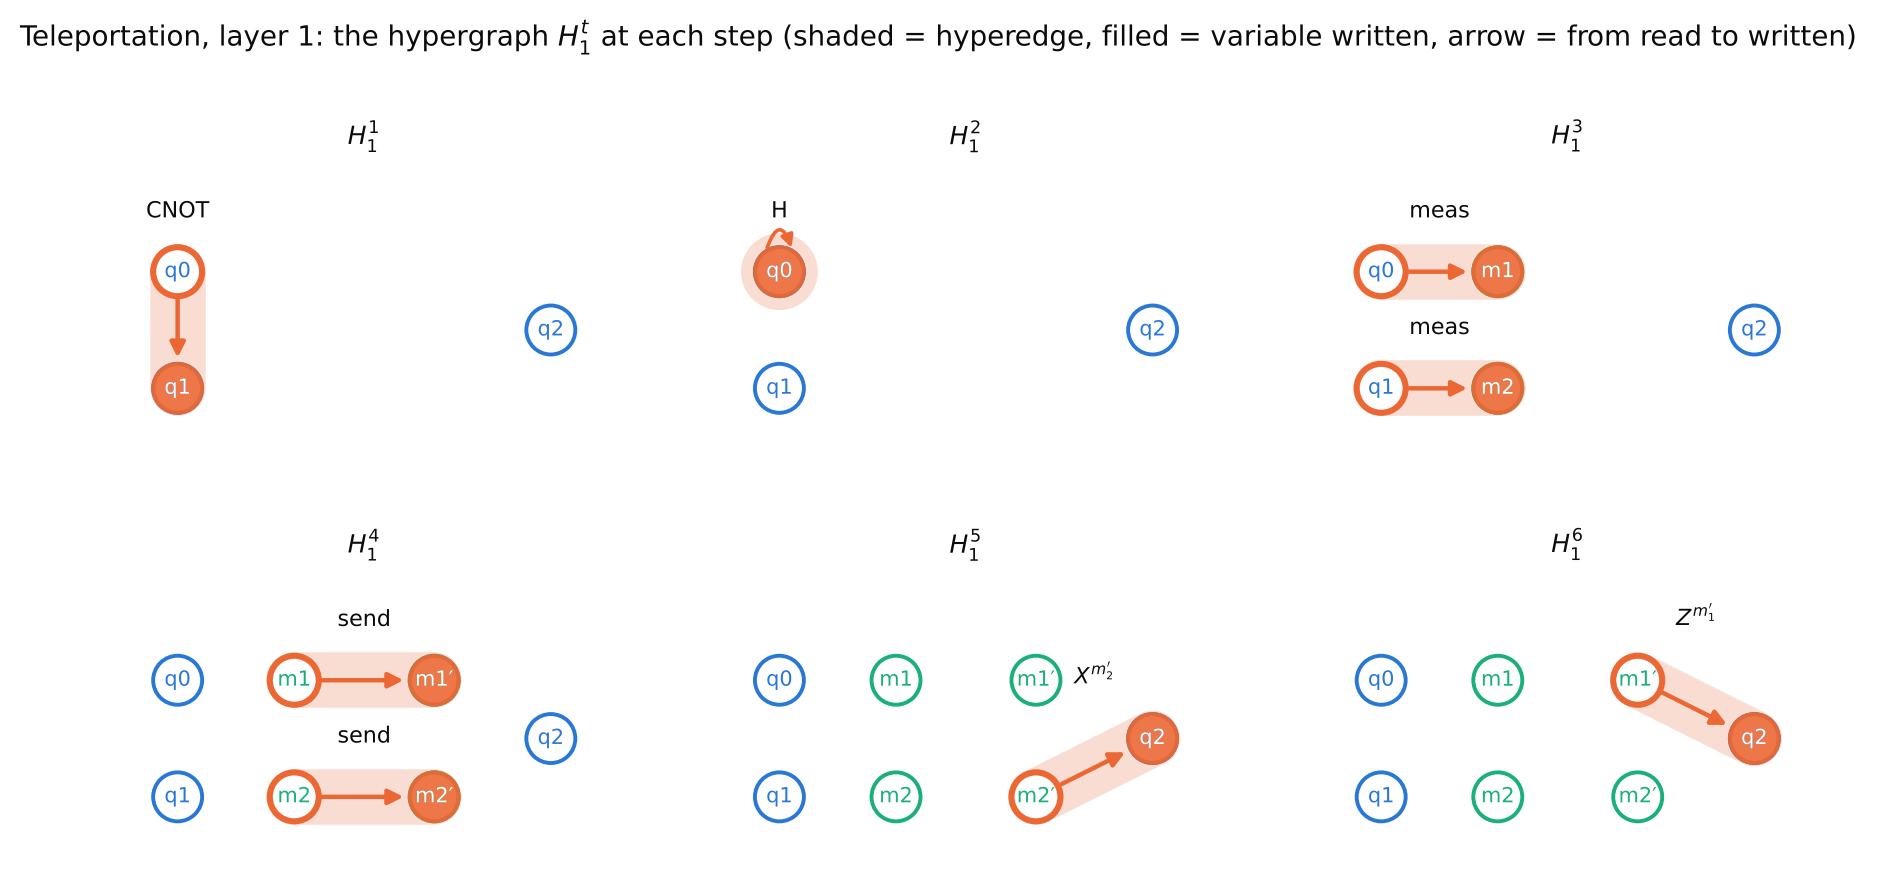
\includegraphics[width=\textwidth]{figs_constructions/tele_layer1_hg.png}

\textit{Figure 4. Layer 1 of teleportation: the hypergraph $H_1^t$ at each step $t=1,\dots,6$, on fixed vertex positions. Shaded region: hyperedge; orange ring: variable read; orange fill: variable written; arrow: from read to written.}
\end{center}

\paragraph{The sheaf.} Before step $3$ all variables are qubits, and $\mathcal{F}(\sigma)$ is the set of density operators on $\bigotimes_{v\in\sigma}\mathbb{C}^2$, with $\rho_{\sigma\tau}$ the partial trace. From step $3$ on, the variables are mixed, and $\mathcal{F}(\sigma)$ is the set of classical--quantum states: block-diagonal operators $\sum_m p(m)\,|m\rangle\langle m|\otimes\rho_m$, one quantum block per value $m$ of the classical variables in $\sigma$. The restriction traces out qubits and sums out classical values. At $t=0$ the local states are those computed for layer $0$: $s_0|_{q_1q_2}=|\beta_{00}\rangle\langle\beta_{00}|$, while $s_0|_{q_1}=s_0|_{q_2}=I/2$, so each half of the Bell pair is completely random on its own.

\paragraph{The dynamics.} Write $|\psi\rangle=\alpha|0\rangle+\beta|1\rangle$. The global states are those of Nielsen--Chuang, \S1.3.7.

Each step below acts only on the vertices of the hyperedges in the panel $H_1^t$ of Figure 4. $\Phi_1$ applies $\mathrm{CNOT}$ to $q_0q_1$:
\[ s_1=\tfrac{1}{\sqrt2}\big(\alpha|0\rangle(|00\rangle+|11\rangle)+\beta|1\rangle(|10\rangle+|01\rangle)\big). \]
$\Phi_2$ applies $H$ to $q_0$; regrouping by the values of $q_0q_1$,
\[ s_2=\tfrac12\Big(|00\rangle(\alpha|0\rangle+\beta|1\rangle)+|01\rangle(\alpha|1\rangle+\beta|0\rangle)+|10\rangle(\alpha|0\rangle-\beta|1\rangle)+|11\rangle(\alpha|1\rangle-\beta|0\rangle)\Big), \]
where the last factor is the state of $q_2$. Each of the four factors is $X^{m_2}Z^{m_1}|\psi\rangle$ for the corresponding values $m_1m_2$ of $q_0q_1$.

$\Phi_3$ is the measurement channel on $q_0$ and $q_1$, which records the outcomes in $m_1,m_2$: each outcome has probability $1/4$, and
\[ s_3|_{m_1m_2q_2}=\sum_{m_1,m_2}\tfrac14\,|m_1m_2\rangle\langle m_1m_2|\otimes X^{m_2}Z^{m_1}|\psi\rangle\langle\psi|Z^{m_1}X^{m_2}. \]
$\Phi_4$ copies $m_1,m_2$ into $m_1',m_2'$. $\Phi_5$ applies $X$ to $q_2$ in the blocks where $m_2'=1$, which removes the $X^{m_2}$; $\Phi_6$ applies $Z$ where $m_1'=1$, which removes the $Z^{m_1}$. Hence
\[ s_6|_{m_1'm_2'q_2}=\Big(\sum_{m_1,m_2}\tfrac14|m_1m_2\rangle\langle m_1m_2|\Big)\otimes|\psi\rangle\langle\psi|. \]

\paragraph{Evolution through time.} Reading correlations off the local states $s_t|_\sigma$ shows what the dynamics does to the relations of layer $0$; Figure 5 draws them, one panel per stage, with line width proportional to the mutual information. Let $H_2(p)=-p\log_2p-(1-p)\log_2(1-p)$.
\begin{center}
\begin{tabular}{llll}
\hline
after step & $I(q_0{:}q_1)$ & $I(q_0{:}q_2)$ & $I(q_1{:}q_2)$\\
\hline
$0$ (layer $0$) & $0$ & $0$ & $2$\\
$1$ (CNOT) & $H_2(|\alpha|^2)$ & $H_2(|\alpha|^2)$ & $2-H_2(|\alpha|^2)$\\
$2$ (H) & unchanged & unchanged & unchanged\\
\hline
\end{tabular}
\end{center}
These values were computed for two random states $|\psi\rangle$ and agree with the formulas to four decimals; the Hadamard acts on $q_0$ alone and cannot change any of them. After the measurements, the bits share exactly one bit with Bob's qubit, $I(m_1m_2{:}q_2)=1$: given the bits, $q_2$ is in a known pure state, and without them it is $I/2$. After the corrections, $I(m_1'm_2'{:}q_2)=0$ and $q_2$ is in $|\psi\rangle$. Layer $1$ shows the route the correlation takes: from the edge $\{q_1,q_2\}$ of layer $0$, through the CNOT on $\{q_0,q_1\}$, into the measured bits, across the channel, and back onto $q_2$ through the two correction hyperedges. Put Figures 4 and 5 side by side: each change between two panels of Figure 5 is produced by the hyperedges of the corresponding panel of Figure 4, and only on their vertices.

\begin{center}
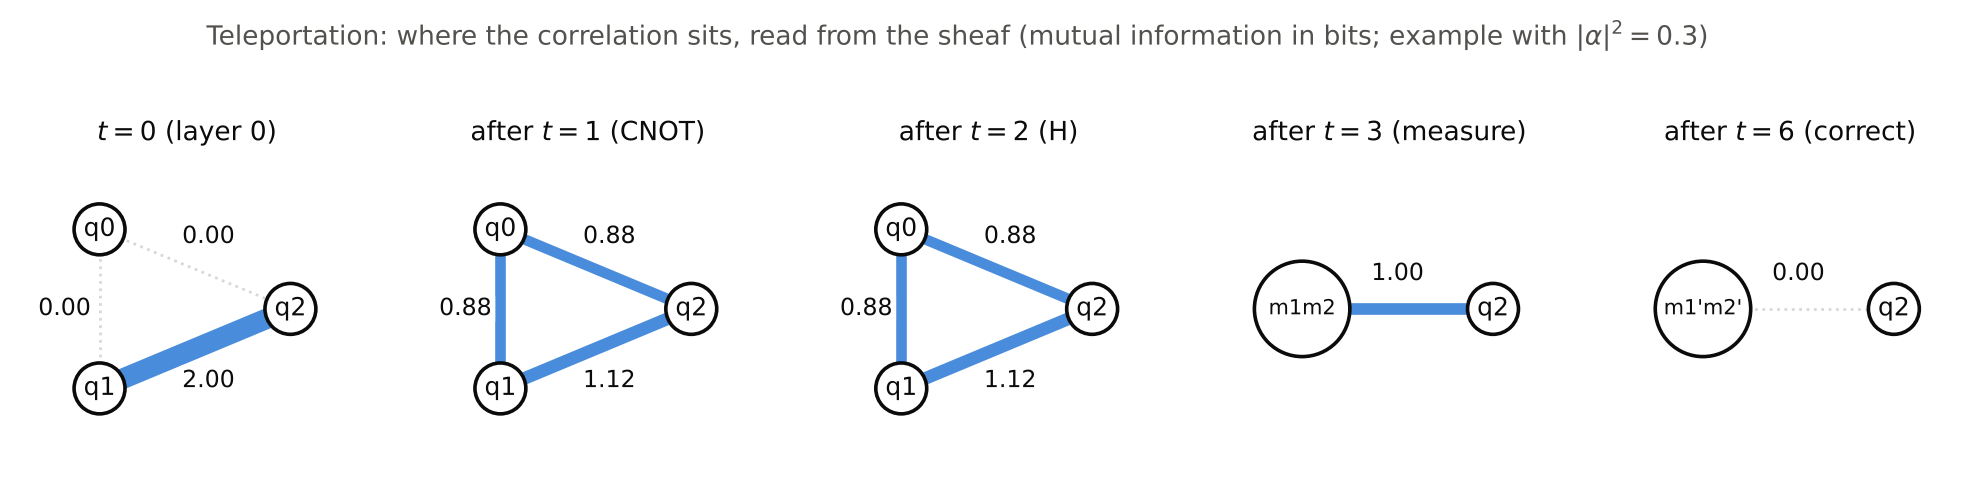
\includegraphics[width=\textwidth]{figs_constructions/tele_correlations.png}

\textit{Figure 5. Where the correlation sits during teleportation, read from the local states of the sheaf. Line width is proportional to the mutual information. The two bits of correlation of the Bell pair are spread over the three qubits by the CNOT, unchanged by the Hadamard, concentrated into one bit between the measured outcomes and Bob's qubit, and removed by the corrections.}
\end{center}

\subsection{A3. BB84, one round, with an intercept--resend eavesdropper}

\paragraph{Variables and domains.} The input variables are the four random bits and the qubit: $V_{in}=\{a,\alpha,\varepsilon,\beta,q\}$, with domains $\{0,1\}$ and $\mathbb{C}^2$. The run creates $e$ (Eve's outcome), $r$ (Bob's outcome), the copies $\alpha',\beta'$, the comparison bits $\kappa_A,\kappa_B$, the kept bits $s_A,s_B$, the copy $s_A'$ and the error bit $\mathit{err}$, all in $\{0,1\}$. The variable $q$ is the same qubit throughout: Eve's resent qubit replaces it.

\paragraph{Schedule.} Thirteen steps: Alice's two gates, Eve's four actions, Bob's gate and measurement, the announcement of the bases, the two comparisons, the two kept bits, the announcement of $s_A$, and the error bit. The two announcements, the two comparisons and the two kept bits are each made at the same time by the two parties.

\paragraph{Layer 0.} The four bits are independent and uniform, and $q$ starts in $|0\rangle$. A classical distribution is a diagonal density operator, so the weights are computed as for qubits: the input state is a product, every reduced state is a product, and every weight is $0$. Layer $0$ has five vertices and no hyperedge: all the structure of BB84 is created by the protocol.

\paragraph{Layer 1.}
\begin{center}
\begin{tabular}{lll}
\hline
step & hyperedges & term\\
\hline
$1$ & $\{a,q\}\to q$ & $X^{a}$\\
$2$ & $\{\alpha,q\}\to q$ & $H^{\alpha}$\\
$3$ & $\{\varepsilon,q\}\to q$ & $H^{\varepsilon}$\\
$4$ & $\{q\}\to e$ & measurement\\
$5$ & $\{e\}\to q$ & reset and $X^{e}$\\
$6$ & $\{\varepsilon,q\}\to q$ & $H^{\varepsilon}$\\
$7$ & $\{\beta,q\}\to q$ & $H^{\beta}$\\
$8$ & $\{q\}\to r$ & measurement\\
$9$ & $\{\alpha\}\to\alpha'$,\ \ $\{\beta\}\to\beta'$ & copy\\
$10$ & $\{\alpha',\beta\}\to\kappa_B$,\ \ $\{\alpha,\beta'\}\to\kappa_A$ & equality test\\
$11$ & $\{\kappa_A,a\}\to s_A$,\ \ $\{\kappa_B,r\}\to s_B$ & keep if equal\\
$12$ & $\{s_A\}\to s_A'$ & copy\\
$13$ & $\{s_A',s_B\}\to\mathit{err}$ & inequality test\\
\hline
\end{tabular}
\end{center}
Step $5$ is one operation: the resent qubit depends only on $e$, so it reads $e$ and writes $q$.\footnote{Modelling choice: Eve's reset followed by $X^{e}$ is taken as one operation.} Steps $4$ and $5$ have the same vertex set $\{q,e\}$ with opposite directions: measuring reads the qubit and writes the bit, resending reads the bit and writes the qubit. Only the direction tells them apart. The comparisons at step $10$ read two variables at once, so their hyperedges have three vertices. Figure 6 draws the hypergraph $H_1^t$ of each step in the convention of Figure 4, with Alice's variables on the left, Eve's at the top and Bob's on the right. In every panel from $H_1^1$ to $H_1^8$ the qubit $q$ belongs to the hyperedge; the panels $H_1^4$ and $H_1^5$ show the same two vertices $q$ and $e$ with the ring and the fill swapped, which is the only difference between Eve's measurement and her resending; from $H_1^9$ on, the hyperedges link Alice's side to Bob's across the public channel and never touch $q$.

\begin{center}
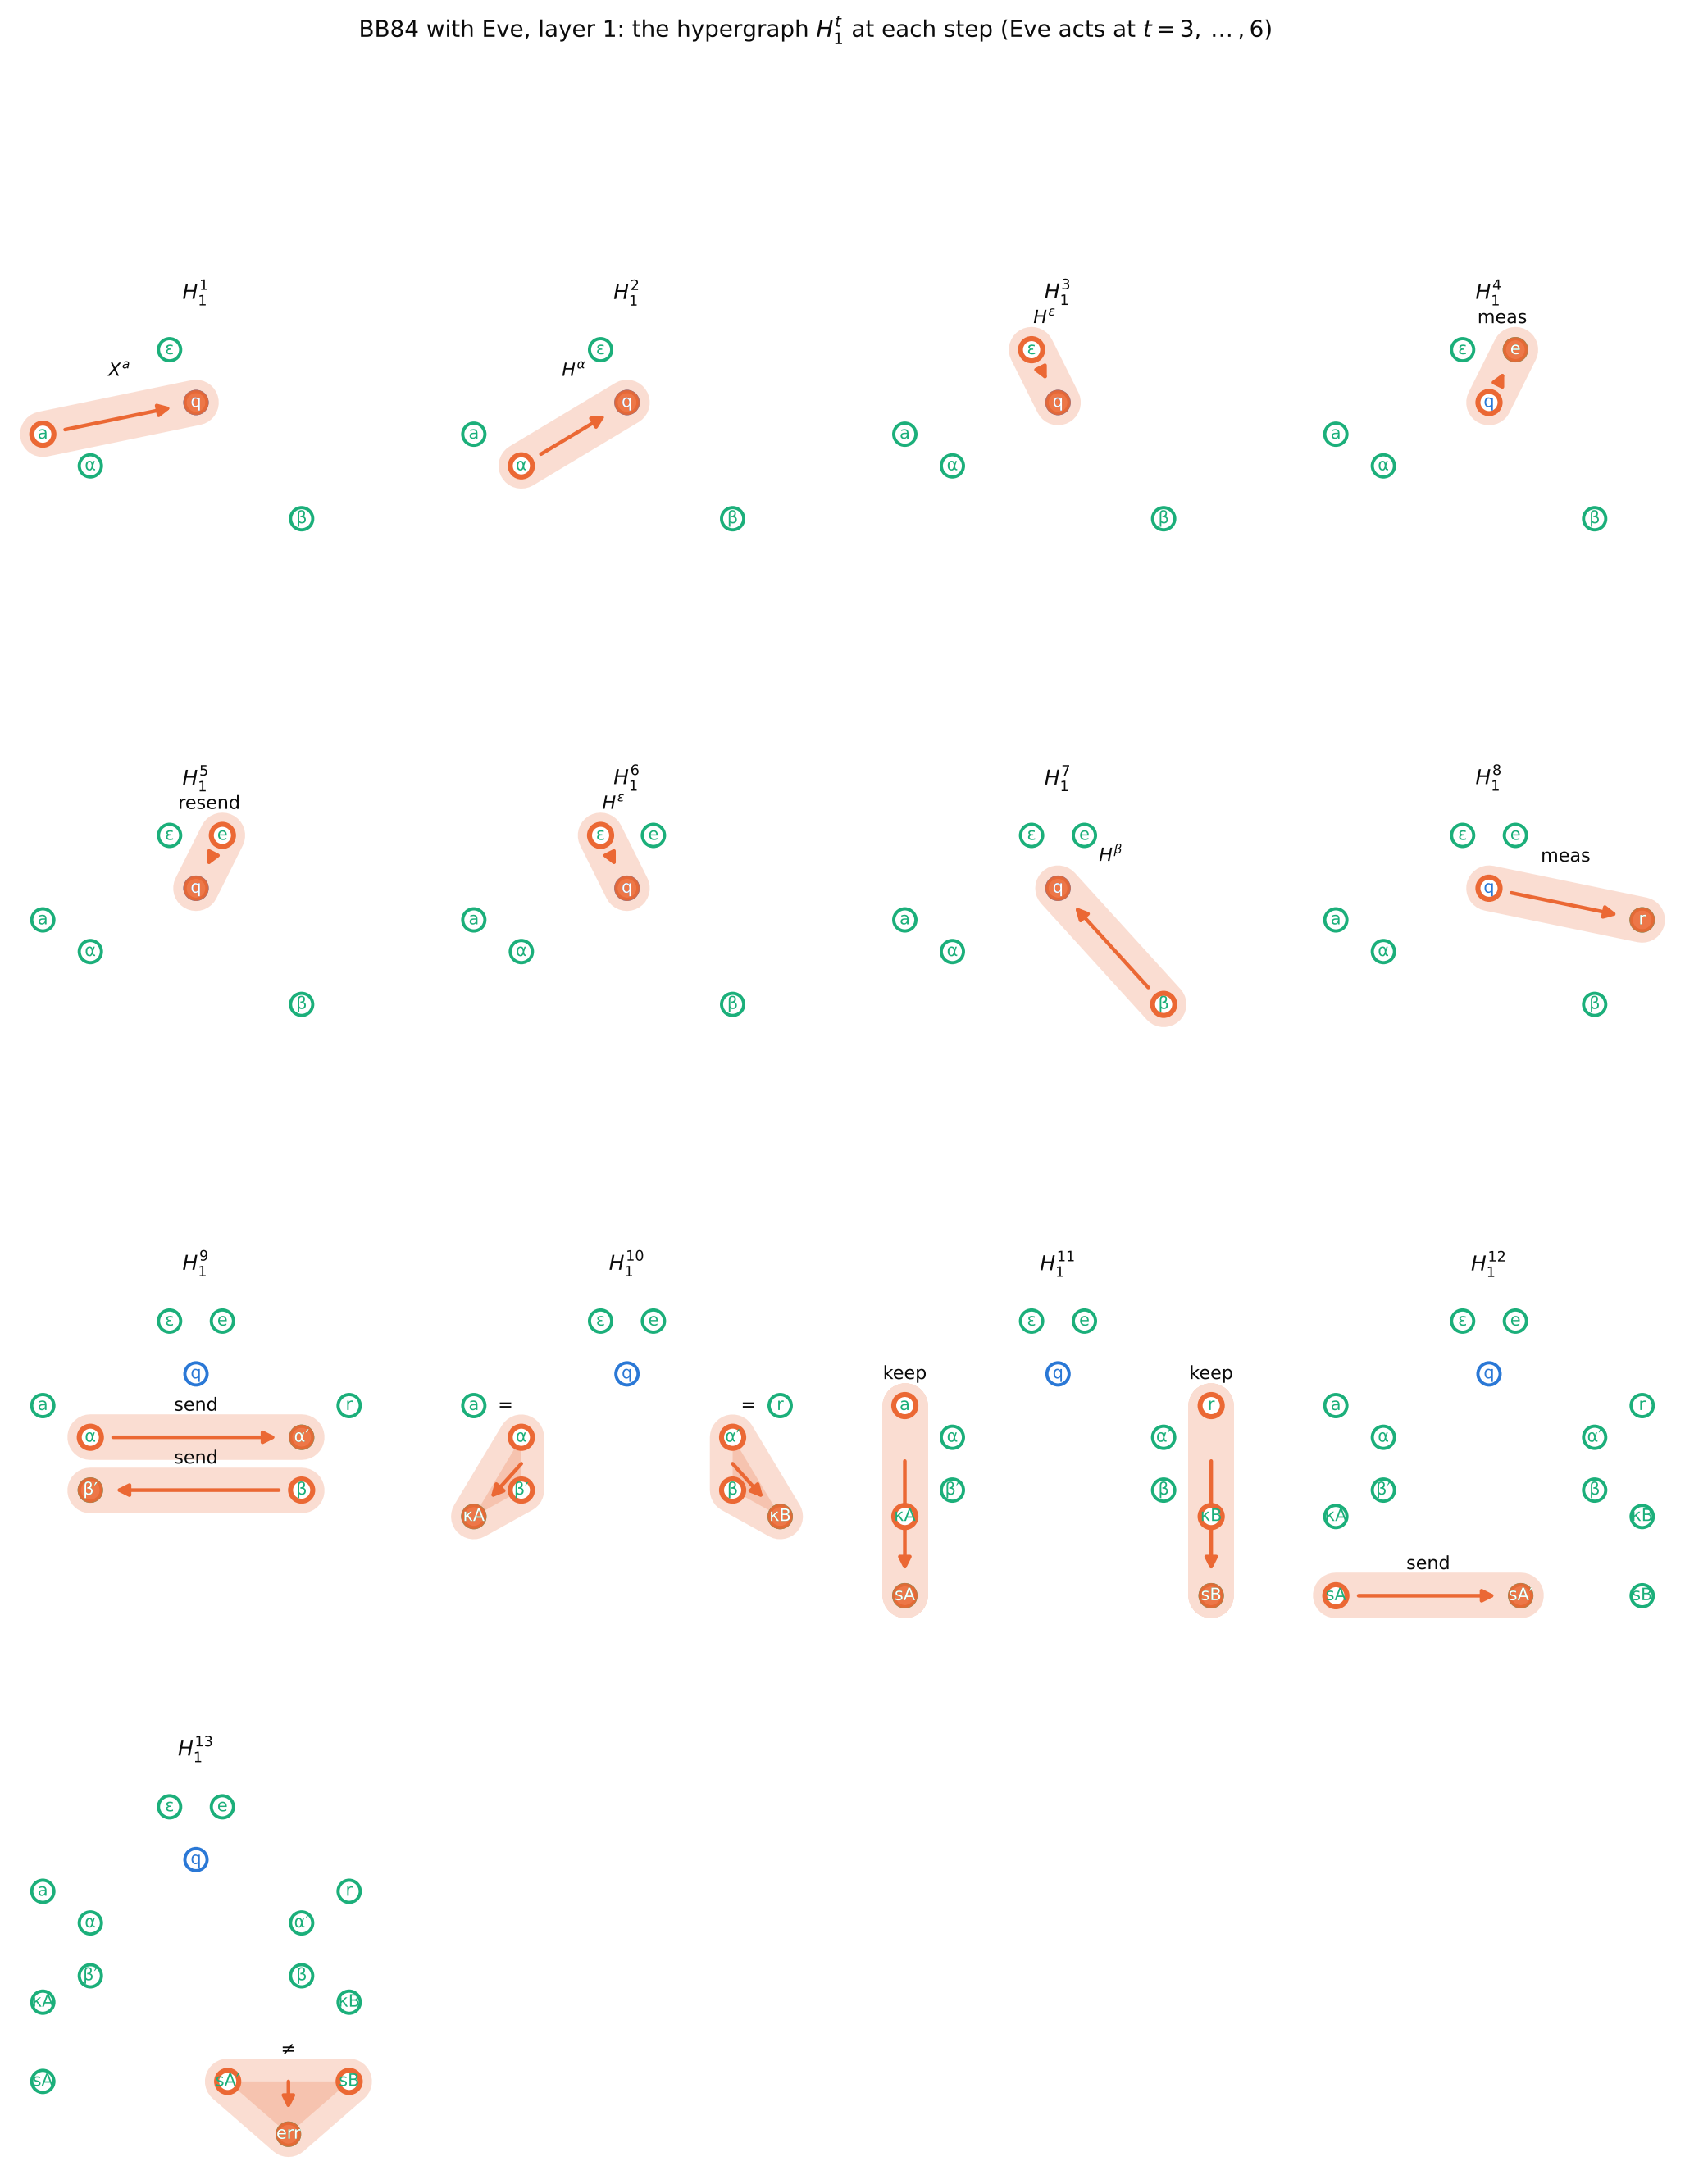
\includegraphics[width=\textwidth]{figs_constructions/bb84_layer1_hg.png}

\textit{Figure 6. Layer 1 of BB84 with Eve: the hypergraph $H_1^t$ at each step $t=1,\dots,13$, drawn as in Figure 4. Alice's variables are on the left, Eve's at the top, Bob's on the right.}
\end{center}

\paragraph{The sheaf.} The variables are mixed, so $\mathcal{F}(\sigma)$ is the set of classical--quantum states on $\sigma$, with restriction by partial trace and summing out.

A restriction already says something at step $2$. After Alice's two gates,
\[ s_2|_{a\alpha q}=\sum_{a,\alpha}\tfrac14\,|a\alpha\rangle\langle a\alpha|\otimes H^{\alpha}X^{a}|0\rangle\langle0|X^{a}H^{\alpha}, \]
whose four blocks are $|0\rangle,|1\rangle,|+\rangle,|-\rangle$. Restricting to $q$ alone sums out $a$ and $\alpha$:
\[ s_2|_{q}=\tfrac14\big(|0\rangle\langle0|+|1\rangle\langle1|+|+\rangle\langle+|+|-\rangle\langle-|\big)=\tfrac12 I. \]
To anyone who holds only the qubit, as Eve does, it is completely random.

Figure 7 shows this restriction geometrically. There, each single-qubit state is a point of the Bloch sphere (Nielsen--Chuang, \S1.2); the four states Alice can send lie on one great circle, and the maximally mixed state $I/2$ is its centre. Restricting to $q$ averages the four points with equal weights, which gives the centre.

\begin{center}
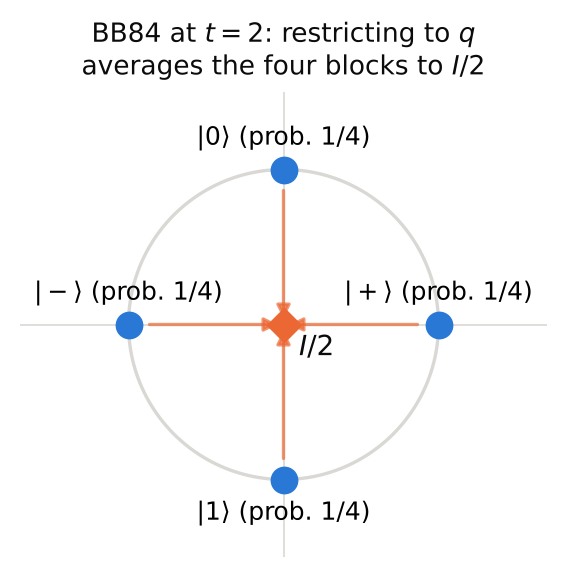
\includegraphics[width=0.45\textwidth]{figs_constructions/bb84_restriction.png}

\textit{Figure 7. The restriction map at work: summing out $a$ and $\alpha$ sends the four blocks of $s_2|_{a\alpha q}$ to their average $I/2$.}
\end{center}

\paragraph{The dynamics.} Follow the classical record and the qubit block by block. After step $4$: if $\varepsilon=\alpha$, Eve measured in the basis Alice used and $e=a$ with certainty; if $\varepsilon\neq\alpha$, she measured in the other basis and $e$ is uniform. After steps $5$ and $6$, $q$ is in the state $H^{\varepsilon}X^{e}|0\rangle$, prepared by Eve. After step $8$: if $\beta=\varepsilon$, $r=e$; otherwise $r$ is uniform. Steps $9$ to $11$ produce $\kappa_A=\kappa_B=[\alpha=\beta]$, and $s_A=a$, $s_B=r$ on the rounds with $\kappa=1$. On those rounds, enumerating the sixteen values of $(a,\alpha,\varepsilon,\beta)$ gives
\[ \Pr(\mathit{err}=1\mid\kappa=1)=\tfrac14, \]
while without Eve (steps $3$ to $6$ removed) the same computation gives $0$. Bases agree in half the rounds. These are the standard values for intercept--resend (Nielsen--Chuang, \S12.6.3). Figure 8 shows the local state $s_{13}|_{\mathit{err}}$ on the rounds with $\kappa=1$, with and without Eve's four hyperedges (panels $H_1^3$ to $H_1^6$ of Figure 6).

\begin{center}
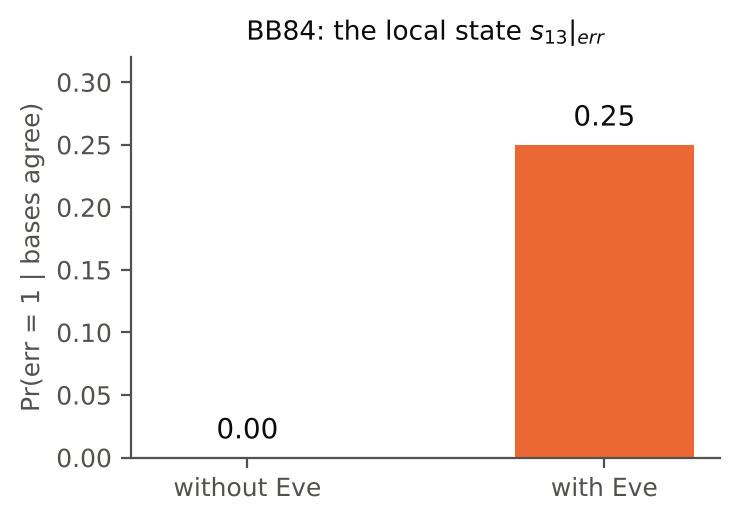
\includegraphics[width=0.5\textwidth]{figs_constructions/bb84_error.png}

\textit{Figure 8. The local state of the error bit on rounds where the bases agree: Eve's four operations leave a trace of one quarter.}
\end{center}

\paragraph{Evolution through time.} Layer $0$ is empty, so every relation of BB84 is created by layer $1$, and layer $1$, as Figure 6 shows, is threaded through a single variable for its first eight steps: every operation from step $1$ to step $8$ touches $q$. Eve's intervention occupies steps $3$ to $6$, and its trace in the classical record is visible only at step $13$, through the local state $s_{13}|_{\mathit{err}}$. From step $9$ on the qubit is no longer touched and the structure is purely classical: two parallel chains, Alice's $\alpha\to\kappa_A\to s_A$ and Bob's $\beta\to\kappa_B\to s_B$, joined by the copies across the public channel and closed by the error test.

\subsection{What the three constructions show}

On BFS, layer $0$ carries the input's whole structure and layer $1$ uses part of it, one relation per step. On teleportation, layer $0$ carries one strong relation, and layer $1$ with the sheaf shows that relation being moved from one pair of variables to another. On BB84, layer $0$ is empty and the whole structure is made by the protocol, with the eavesdropper visible in layer $1$ as a pair of operations on the same vertices in opposite directions, and in the sheaf as an error rate of one quarter. In all three, the sheaf is what turns the hypergraphs into statements about the computation: without it the layers record which variables are related, but not what the relation does.

\end{document}
